\subsection{Módulo genérico de los cambios de vías dobles}
	\label{sec:ACG_dsw}
	
	El módulo \textit{DoubleSwitches} (ver Figura \ref{fig:GeneralSystem}) es el encargado de implementar el funcionamiento de los cambios de vías dobles en la red ferroviaria. Al igual que para el módulo \textit{SingleSwitches}, el ACG utiliza la información otorgada por el RNA para implementar las mismas entradas y salidas en el módulo \textit{DoubleSwitches}. El diagrama de bloques de la máquina de estados finitos con camino de datos diseñado para lograr este objetivo se muestra en la Figura \ref{fig:DSW_module}.
	
	\begin{figure}[H]
		\centering
		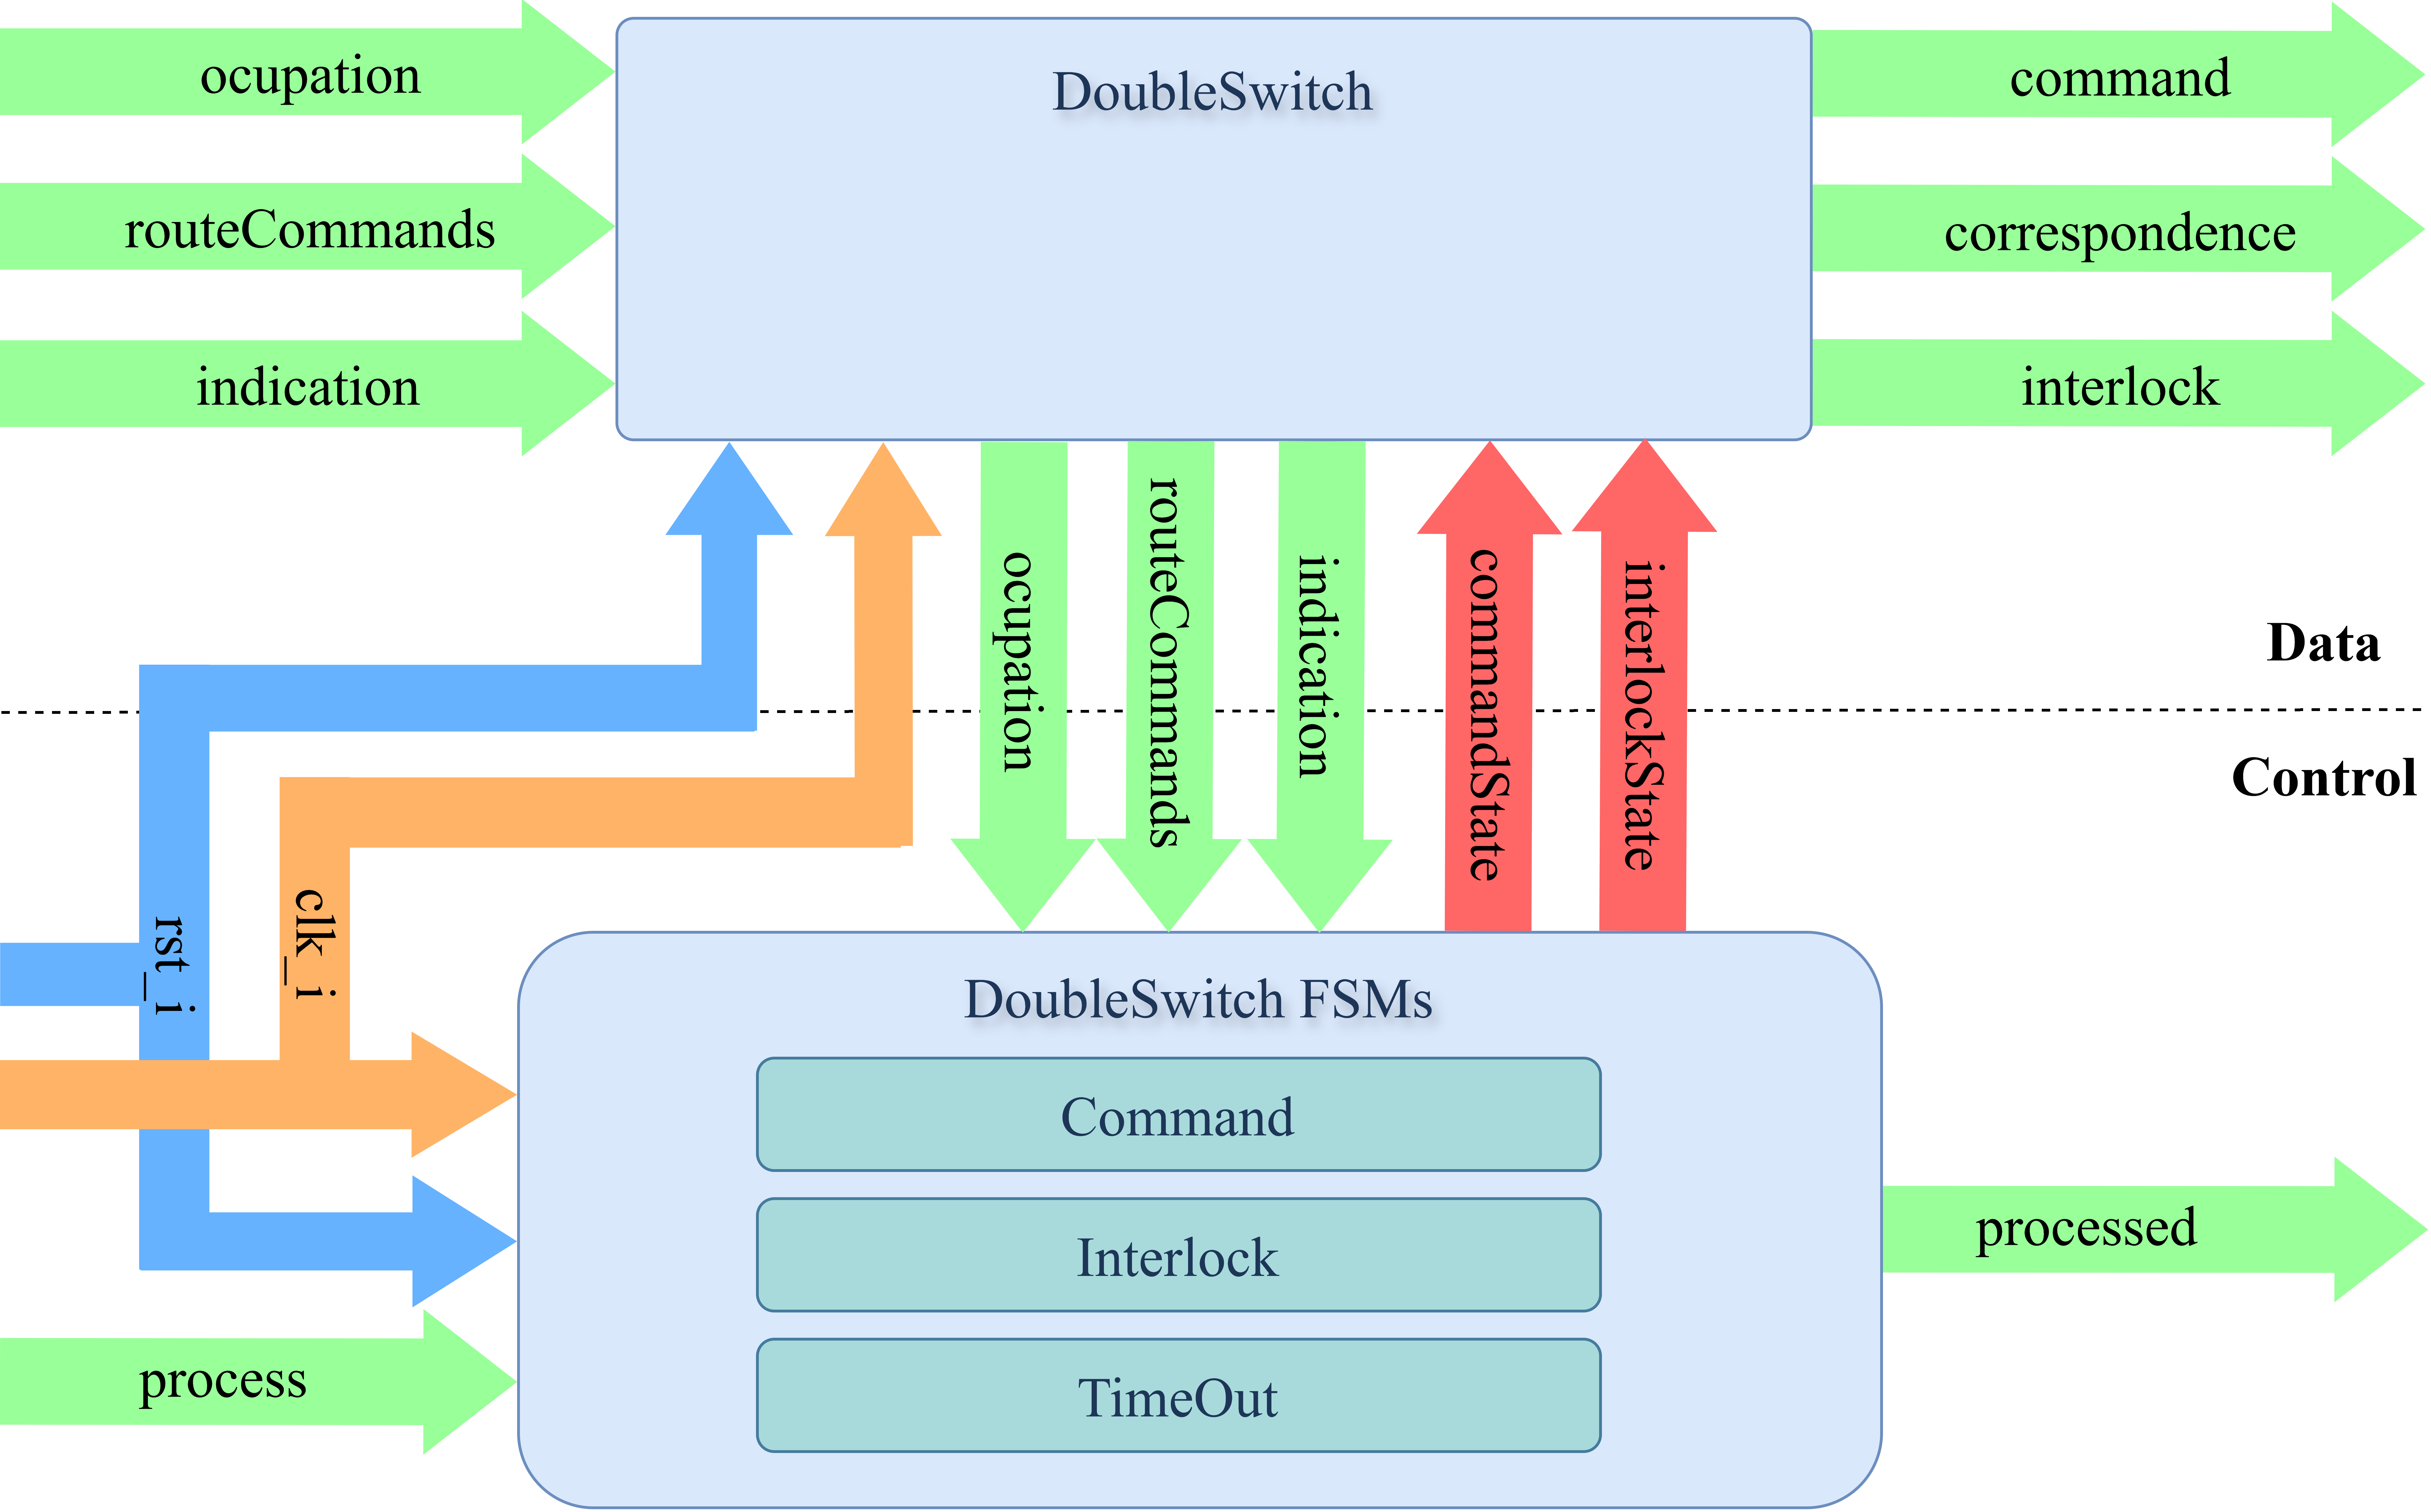
\includegraphics[width=0.8\textwidth]{Figuras/DSW_module}
		\centering\caption{FSMD del módulo genérico de \textit{DoubleSwitches}.}
		\label{fig:DSW_module}
	\end{figure}
	
	Aunque en una primera inspección las Figuras \ref{fig:SSW_module} y \ref{fig:DSW_module} puedan parecer muy similares, la diferencia entre ambos módulos radica en el tipo de datos utilizados en la indicación, comando y correspondencia, ya que los cambios de vías dobles tienen cuatro estados y no dos cómo los cambios de vías simples, tal se explicó en la Sección \textit{SingleSwitches}. Un cambio de vías dobles puede adoptar las posiciones doble normal, doble reverso, normal reverso y reverso normal. Por lo tanto, señales que pueden adoptar dos estados no son suficientes y deben definirse nuevos tipos de datos que utilizan el doble de tamaño para poder definir cuatro estados. Al tener esto en cuenta, el comportamiento de los cambios de vías dobles es mucho más complejo, tal como se define en la red de Petri de la Figura \ref{fig:DSW_Petri}.
	
	\begin{figure}[H]
		\centering
		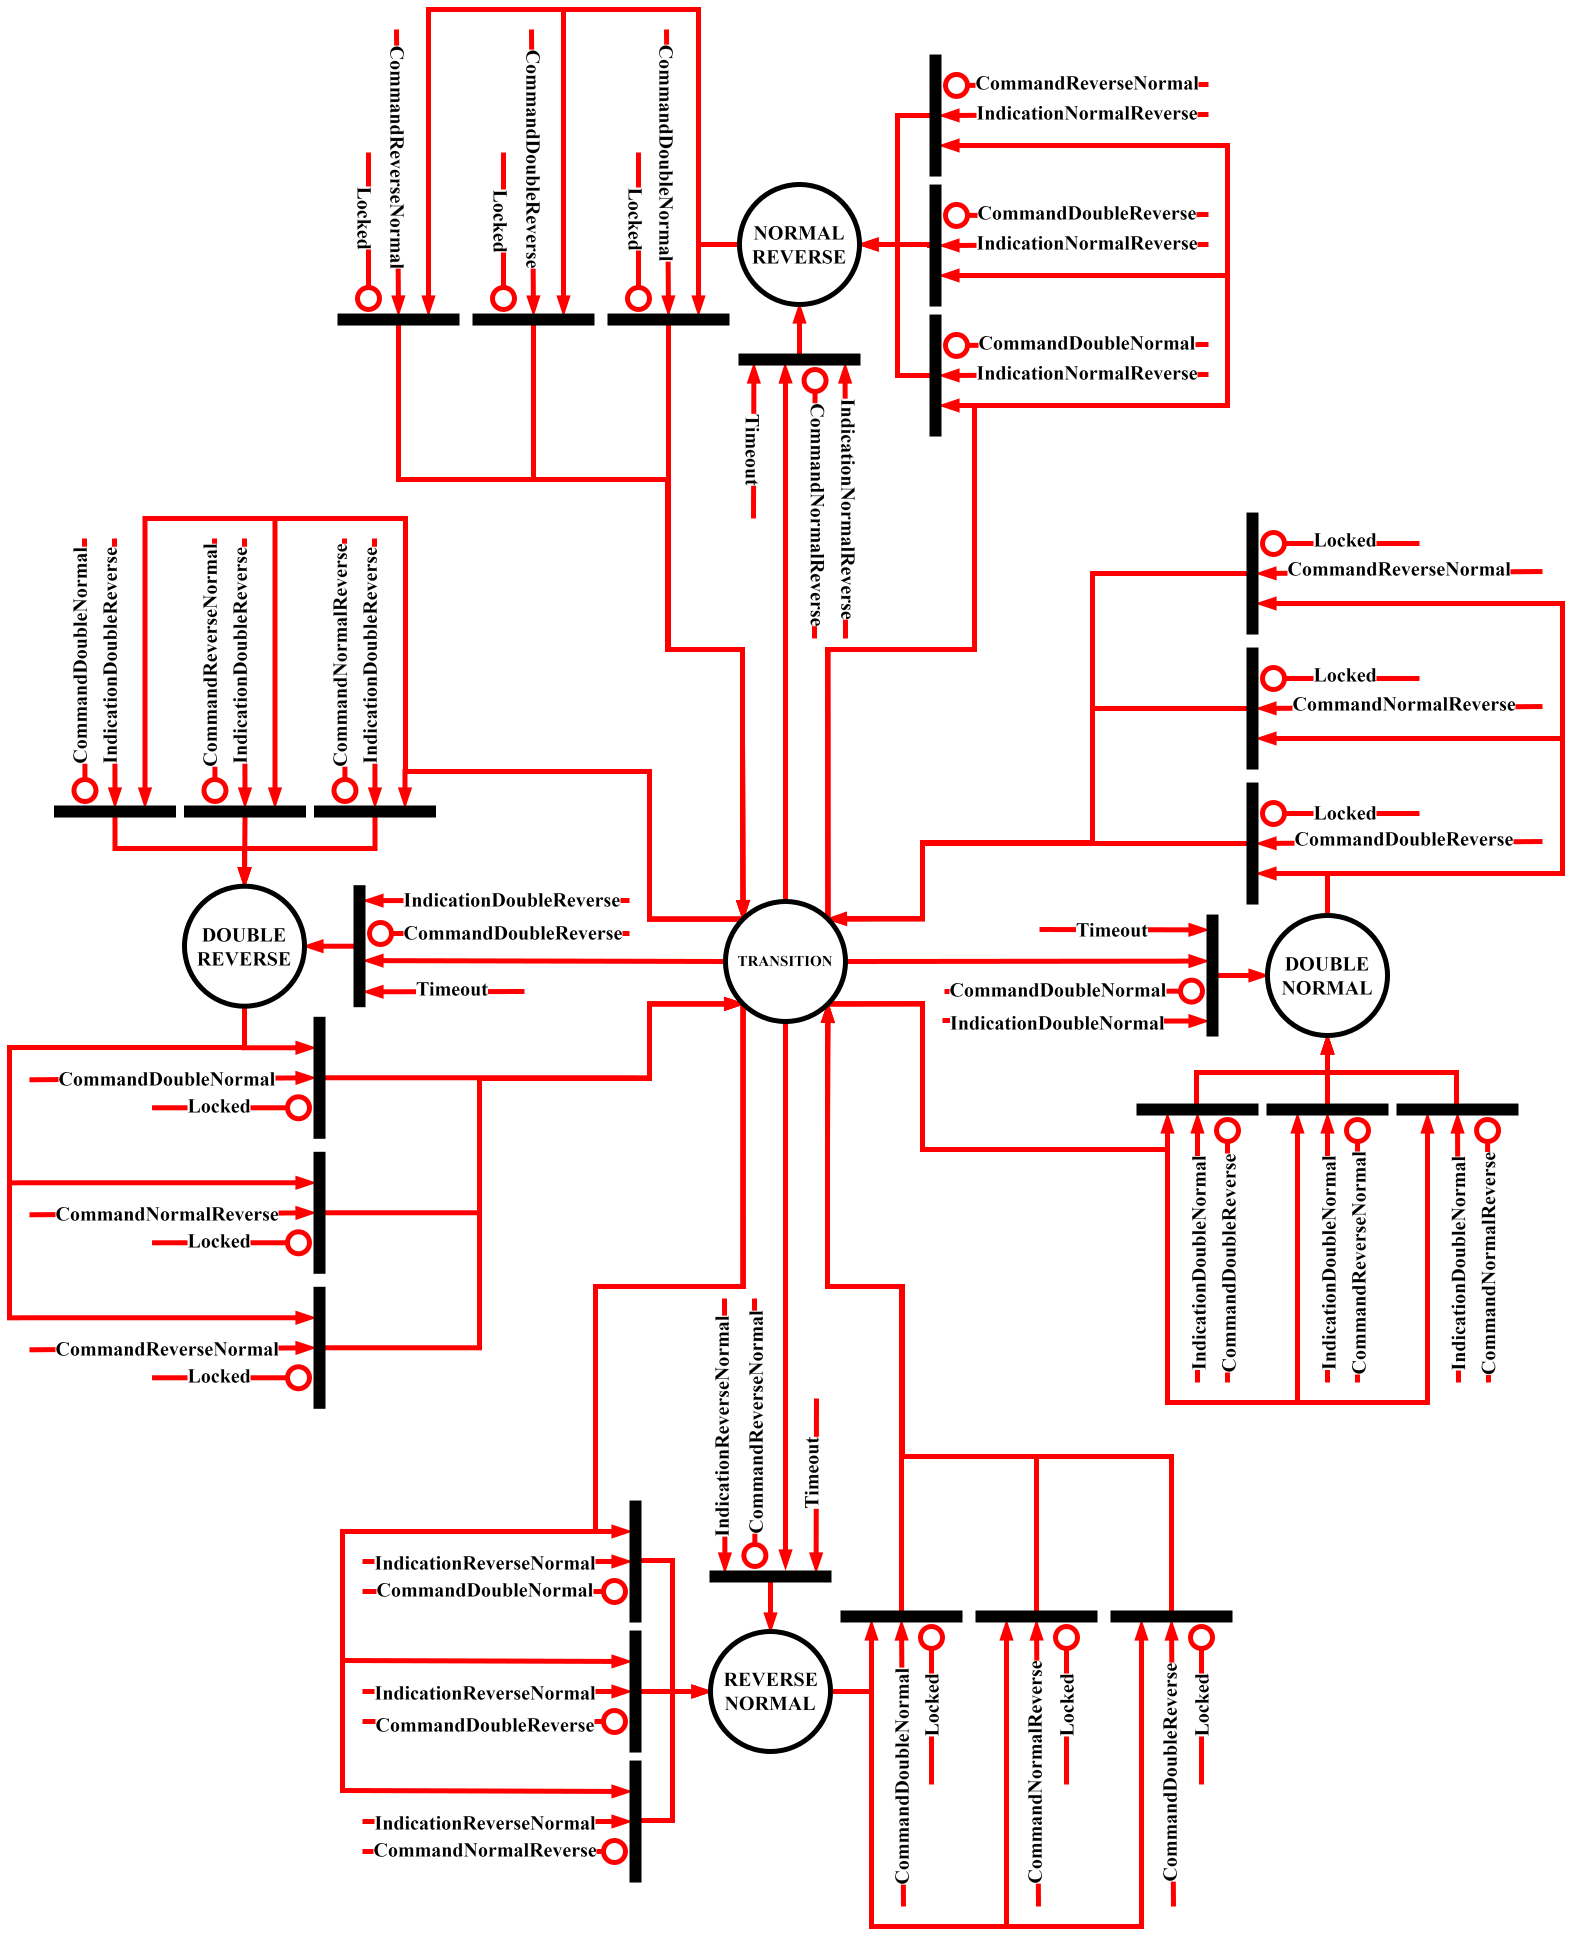
\includegraphics[width=1\textwidth]{Figuras/DSW_petri}
		\centering\caption{Red de Petri del modelo dinámico de \textit{DoubleSwitches}.}
		\label{fig:DSW_Petri}
	\end{figure}
	
	La complejidad de la red de Petri que define el comportamiento del módulo \textit{DoubleSwitches} es mayor que los casos expuestos anteriormente al atenderse una mayor cantidad de posibles transiciones y estados. No obstante, el principio es el mismo que el explicado para el módulo \textit{SingleSwitches}. Cada estado estable pasa al estado de transición sí y solo sí se una ruta envía un comando para que el cambio de vías se desplace a una posición diferente y el cambio de vías no se encuentra enclavado por otra ruta. Una vez en transición, se dispone de una cantidad de tiempo finita (configurable) para completar el movimiento. De no lograrlo, el cambio de vías dobles deberá volver a su posición original, de ser posible. De cumplirse las condiciones adecuadas donde el comando y la indicación coinciden, el cambio de vías dobles alcanza un nuevo estado estable, reportando su posición actual a la ruta que lo solicitó, mediante su correspondencia.
